\chapter{Context and Related Work}
\label{cha:related_work}
\minitoc

\section{Global Warming and ICT Role}
Global warming is one of the most critical environmental issues of our day \cite{houghton2005global}. Global warming is the effect of human activities on the climate, mainly the burning of fossil fuels (coal, oil, and gas) and large-scale deforestation \cite{houghton2005global}. Both activities have grown immensely since the industrial revolution. The burning of fossil fuels process results in greenhouse gas emissions \cite{olabi2022renewable}. Today, fossil fuels are one of the world's main sources of energy production, helping to emit more and more GHG \cite{olabi2022renewable}. GHG stays in the atmosphere creating a layer as a blanket over the planet's surface. Without this blanket, the Earth can balance the radiation energy from the sun and the thermal radiation from the Earth to space \cite{houghton2005global}. However, this human-generated blanket imposes a barrier to the thermal radiation from the Earth, letting it into the atmosphere and heating the planet, working as a greenhouse. All this process works as a greenhouse which is the reason for the name greenhouse gas \cite{houghton2005global}.

This situation brings us to United Nations Climate Change Conference (COP21) in Paris, France, on 12 December 2015. At this conference, 196 signed the Paris Agreement aiming to \cite{nations_paris_nodate}:
\begin{enumerate}
    \item Reduce global greenhouse gas emissions substantially, limiting the global temperature increase in this century to 2\degree C while pursuing measures to limit the growth even further to 1.5\degree C;
    \item Review countries’ commitments every five years (through the Nationally Determined Contribution, or NDC);
    \item Provide financing to developing countries to mitigate climate change, strengthen resilience, and enhance their abilities to adapt to climate impacts. 
\end{enumerate}

These are ambitious but necessary objectives. Since then, countries and organizations have proposed several actions and pledges. However, a recent report indicates that the actual world's effort is not enough \cite{tracker2022projections}. Figure \ref{fig:ghg_cat} shows GHG emission and temperature estimations. We could see that there is a small reduction in emissions increase tendency. Nevertheless, this figure estimates that real-world actions based on current policies will lead to an increase of somewhere between 2.6 and 2.9\degree C by 2100. This estimation is well above the 1.5\degree C pursued by the Paris Agreement. Considering the targets proposed by the countries through NDC, the temperature will be around 2.4\degree C. In a scenario based on NDC targets and submitted and binding long-term targets, the prediction is a temperature of 2\degree C by 2100, the limit proposed by the Paris Agreement. The report forecasts an optimistic scenario analyzing the effect of net zero emissions targets of about 140 countries that are adopted or under discussion. Even in this optimistic scenario, the estimated temperature would be 1.8\degree C. The situation tends to be even worst with the gold rush for gas \cite{tracker2022massive}. The report indicates that in 2022 we arrived at 1.2\degree C warming \cite{tracker2022projections}.

\begin{figure}[!htb]
    \centering
    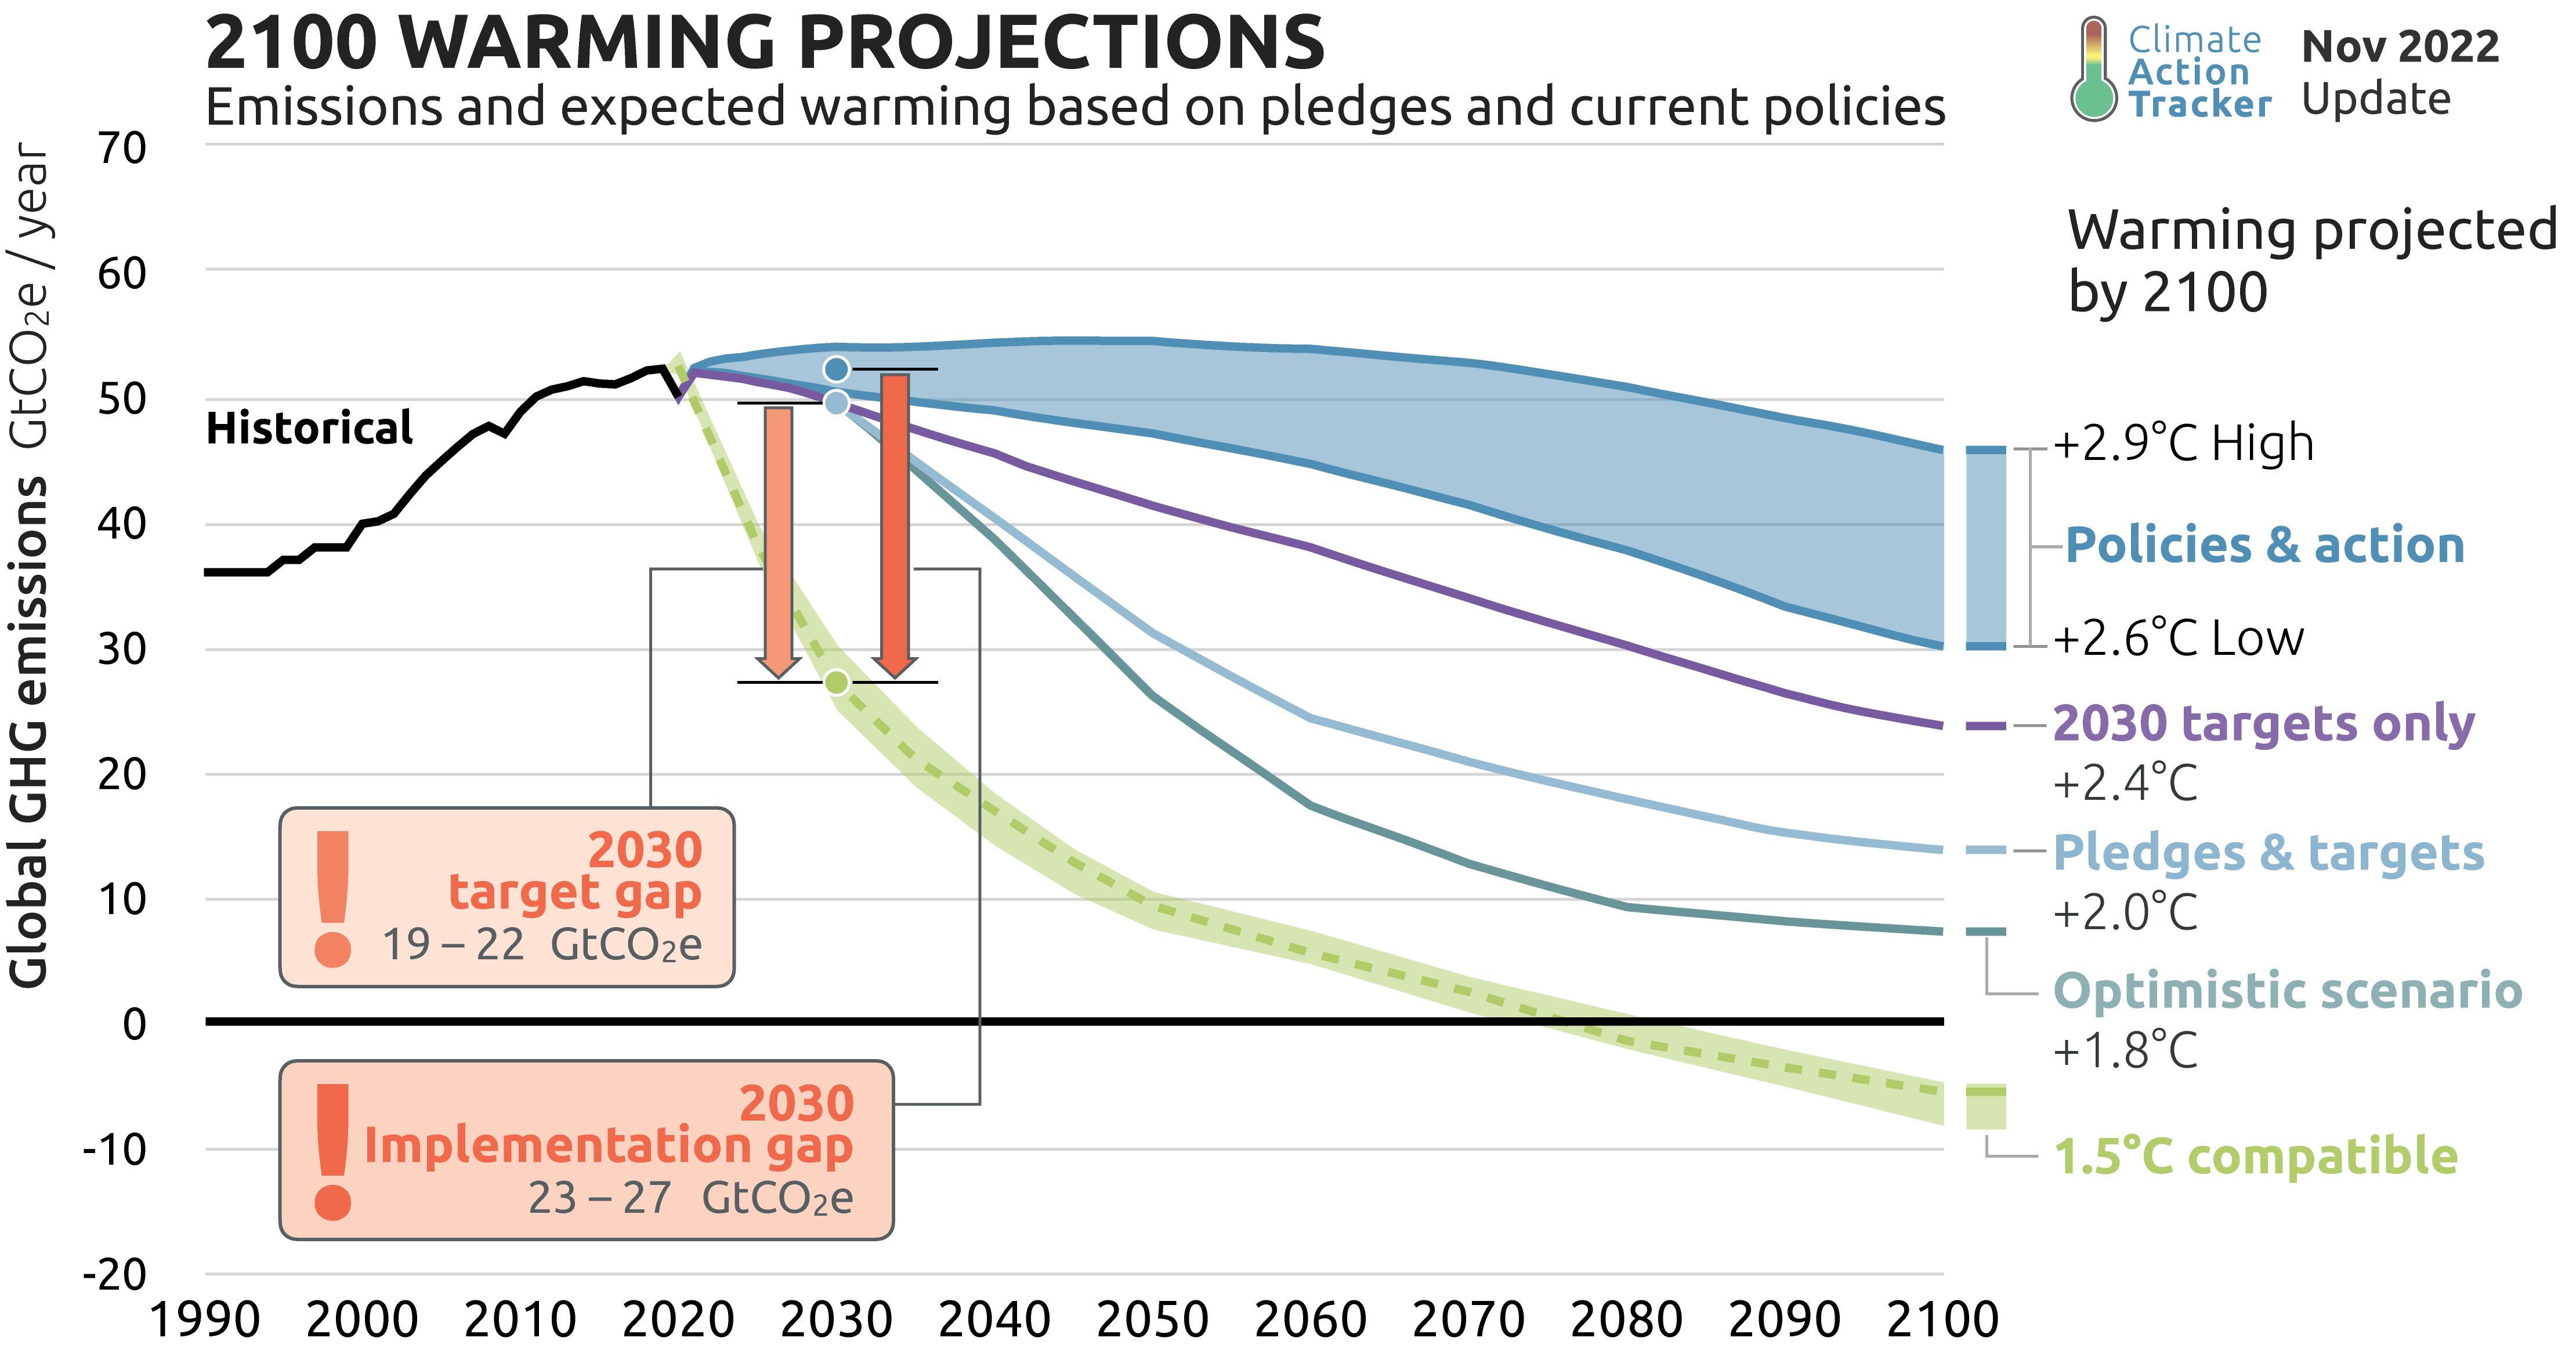
\includegraphics[scale=0.09]{Images/Related_works/Emissions_2022-11.png}
    \caption{Estimated global GHG emissions \cite{tracker2022projections}.}
    \label{fig:ghg_cat}
\end{figure}

We have started to feel the impacts of global warming on humanity, such as heatwaves, droughts, and floods, impacting flora and fauna directly \cite{masson2018global, change2022threat}. In a cascade effect, this increases food and water insecurity worldwide \cite{change2022threat, doi:10.1126/science.1239402}. Also, high temperatures increase mortality, impact labor productivity, impair learning, increase adverse pregnancy outcomes possibility, increase conflict, hate speech, migration, and infectious disease spread \cite{lenton2023quantifying}. Therefore, an increase of the temperature by 2.7\degree C as forecasted would impact one-third (22–39\%) of the world's population by 2100 \cite{lenton2023quantifying}. Climate change has already impacted around 9\% of people (>600 million) \cite{lenton2023quantifying}. Reducing global warming from 2.7 to 1.5\degree C results in a $\sim$5-fold decrease in the population exposed to unprecedented heat (mean annual temperature $\geq$29\degree C) \cite{lenton2023quantifying}. Thus, all sectors must reduce their GHG emissions as much as possible.

Information and Communication Technology is one of these sectors which has accelerated growth in the last 70 years. Unesco defines ICT as \cite{unesco2009guide}:

\begin{quote}
    ``Information and communication technologies (ICT) is defined as a diverse set of technological tools and resources used to transmit, store, create, share or exchange information. These technological tools and resources include computers, the Internet (websites, blogs and emails), live broadcasting technologies (radio, television and webcasting), recorded broadcasting technologies (podcasting, audio and video players, and storage devices) and telephony (fixed or mobile, satellite, visio/video-conferencing, etc.).''
\end{quote}

Regarding the ICT role in GHG emissions, its current global share is around 1.8\%-2.8\%, or 2.1\%-3.9\% considering the supply chain pathways.

% \begin{itemize}
%     \item Present the numbers of global warming generally;
%     \item Present the predictions about the global warming;
%     \item Introduce the role of ICT generally;
%     \item Write about data center impact;
% \end{itemize}

\section{Renewable Energy}
\begin{itemize}
    \item Explain the possible sources of renewable energy;
    \item Show that Renewable energy is a possible way to reduce the global warming problem;
    \item Write about the uncertainties;
\end{itemize}

\section{Renewable-only Data center}
\begin{itemize}
    \item Explain the possibility of applying renewable in data centers;
    \item Show that some big cloud providers are doing it, but not entirely;
    \item Present the challenges in a renewable-only data center;
\end{itemize}

\subsection{Electrical elements}
\begin{itemize}
    \item Write about wind turbines;
    \item Write about solar panel;
    \item Write about battery;
    \item Write about hydrogen;
\end{itemize}

\subsection{IT elements}
\begin{itemize}
    \item Write about the servers;
    \item Write about the power consumption (e.g., DVFS, on-off, idle, etc);
    \item Write about the jobs (e.g., types, resources demanded, etc);
\end{itemize}

\section{Sources of Uncertainty}

\subsection{Weather Uncertainties}
\begin{itemize}
    \item Describe wind uncertainty;
    \item Describe solar irradiation uncertainty;
    \item Describe temperature uncertainty;
\end{itemize}

\subsection{Workload Uncertainties}
\begin{itemize}
    \item Describe job arrival uncertainty;
    \item Describe job size uncertainty;
\end{itemize}

\subsection{Optimization Strategies for Dealing with Uncertainties}
\begin{itemize}
    \item Write about weather predictions
    \item Write about optimization for the weather;
    \item Write about scheduling algorithms to deal with workload uncertainties;
    \item Write about mixing both renewable production and workload uncertainties;
\end{itemize}

\section{Literature Review}

\begin{itemize}
    \item Present the 20 articles selected;
    \item Present a table with each article and the following points:
    \begin{itemize}
        \item Name;
        \item Year;
        \item Source of power (solar, wind, battery, grid, etc);
        \item Level of decision (offline, online, both);
        \item Power adaptations (battery compensations, renewable adaptations, etc).
    \end{itemize}
\end{itemize}

\subsection{Discussion and Classification of the Literature}